\section{mr::disk\-Sampler Class Reference}
\label{classmr_1_1diskSampler}\index{mr::diskSampler@{mr::diskSampler}}
Sample in a disk.  


{\tt \#include $<$mr\-Sampler.h$>$}

Inheritance diagram for mr::disk\-Sampler::\begin{figure}[H]
\begin{center}
\leavevmode
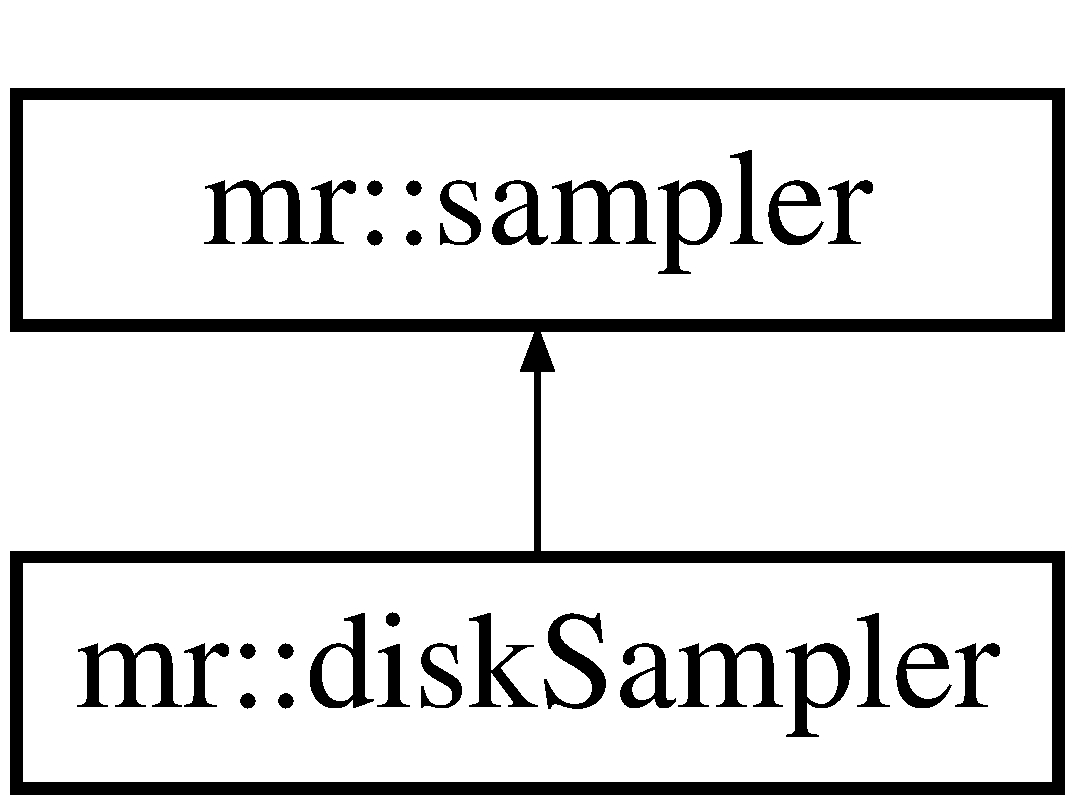
\includegraphics[height=2cm]{classmr_1_1diskSampler}
\end{center}
\end{figure}
\subsection*{Public Member Functions}
\begin{CompactItemize}
\item 
{\bf disk\-Sampler} ()
\item 
{\bf disk\-Sampler} (const mi\-Uint \&num\-Samples)
\item 
{\bf $\sim$disk\-Sampler} ()
\item 
bool {\bf uniform} (const mi\-State $\ast$const)
\begin{CompactList}\small\item\em Get one sample using a uniform distribution or return false. \item\end{CompactList}\item 
bool {\bf concentric} (const mi\-State $\ast$const)
\begin{CompactList}\small\item\em Get one sample using a concentric distribution or return false. \item\end{CompactList}\item 
const mi\-Vector2d \& {\bf position} ()
\begin{CompactList}\small\item\em Return u,v position of sample. \item\end{CompactList}\end{CompactItemize}
\subsection*{Protected Member Functions}
\begin{CompactItemize}
\item 
void {\bf concentric\-Distribution} ()
\item 
void {\bf uniform\-Distribution} ()
\end{CompactItemize}


\subsection{Detailed Description}
Sample in a disk. 



\subsection{Constructor \& Destructor Documentation}
\index{mr::diskSampler@{mr::disk\-Sampler}!diskSampler@{diskSampler}}
\index{diskSampler@{diskSampler}!mr::diskSampler@{mr::disk\-Sampler}}
\subsubsection{\setlength{\rightskip}{0pt plus 5cm}mr::disk\-Sampler::disk\-Sampler ()\hspace{0.3cm}{\tt  [inline]}}\label{classmr_1_1diskSampler_a0}


Constructor. This call is to be used when sampling adaptively (ie. the number of samples to be taken are not known or may vary, or you may exit the loop early). \index{mr::diskSampler@{mr::disk\-Sampler}!diskSampler@{diskSampler}}
\index{diskSampler@{diskSampler}!mr::diskSampler@{mr::disk\-Sampler}}
\subsubsection{\setlength{\rightskip}{0pt plus 5cm}mr::disk\-Sampler::disk\-Sampler (const mi\-Uint \& {\em num\-Samples})\hspace{0.3cm}{\tt  [inline]}}\label{classmr_1_1diskSampler_a1}


Constructor. Fixed Sampling. num\-Samples is the number of samples to take. It HAS to be mi\-Uint\& \index{mr::diskSampler@{mr::disk\-Sampler}!~diskSampler@{$\sim$diskSampler}}
\index{~diskSampler@{$\sim$diskSampler}!mr::diskSampler@{mr::disk\-Sampler}}
\subsubsection{\setlength{\rightskip}{0pt plus 5cm}mr::disk\-Sampler::$\sim${\bf disk\-Sampler} ()\hspace{0.3cm}{\tt  [inline]}}\label{classmr_1_1diskSampler_a2}




\subsection{Member Function Documentation}
\index{mr::diskSampler@{mr::disk\-Sampler}!concentric@{concentric}}
\index{concentric@{concentric}!mr::diskSampler@{mr::disk\-Sampler}}
\subsubsection{\setlength{\rightskip}{0pt plus 5cm}bool mr::disk\-Sampler::concentric (const mi\-State $\ast$ {\em const })\hspace{0.3cm}{\tt  [inline]}}\label{classmr_1_1diskSampler_a4}


Get one sample using a concentric distribution or return false. 

\index{mr::diskSampler@{mr::disk\-Sampler}!concentricDistribution@{concentricDistribution}}
\index{concentricDistribution@{concentricDistribution}!mr::diskSampler@{mr::disk\-Sampler}}
\subsubsection{\setlength{\rightskip}{0pt plus 5cm}void mr::disk\-Sampler::concentric\-Distribution ()\hspace{0.3cm}{\tt  [inline, protected]}}\label{classmr_1_1diskSampler_b0}


\index{mr::diskSampler@{mr::disk\-Sampler}!position@{position}}
\index{position@{position}!mr::diskSampler@{mr::disk\-Sampler}}
\subsubsection{\setlength{\rightskip}{0pt plus 5cm}const mi\-Vector2d\& mr::disk\-Sampler::position ()\hspace{0.3cm}{\tt  [inline]}}\label{classmr_1_1diskSampler_a5}


Return u,v position of sample. 

\index{mr::diskSampler@{mr::disk\-Sampler}!uniform@{uniform}}
\index{uniform@{uniform}!mr::diskSampler@{mr::disk\-Sampler}}
\subsubsection{\setlength{\rightskip}{0pt plus 5cm}bool mr::disk\-Sampler::uniform (const mi\-State $\ast$ {\em const })\hspace{0.3cm}{\tt  [inline]}}\label{classmr_1_1diskSampler_a3}


Get one sample using a uniform distribution or return false. 

\index{mr::diskSampler@{mr::disk\-Sampler}!uniformDistribution@{uniformDistribution}}
\index{uniformDistribution@{uniformDistribution}!mr::diskSampler@{mr::disk\-Sampler}}
\subsubsection{\setlength{\rightskip}{0pt plus 5cm}void mr::disk\-Sampler::uniform\-Distribution ()\hspace{0.3cm}{\tt  [inline, protected]}}\label{classmr_1_1diskSampler_b1}




The documentation for this class was generated from the following file:\begin{CompactItemize}
\item 
{\bf mr\-Sampler.h}\end{CompactItemize}
